\documentclass{article}
\usepackage{amsmath, amsthm, amssymb}
\usepackage{tikz}
% set font encoding for PDFLaTeX, XeLaTeX, or LuaTeX
\usepackage{ifxetex,ifluatex}
\if\ifxetex T\else\ifluatex T\else F\fi\fi T%
  \usepackage{fontspec}
\else
  \usepackage[T1]{fontenc}
  \usepackage[utf8]{inputenc}
  \usepackage{lmodern}
\fi

\usepackage{hyperref}

\newcommand{\CC}{\mathcal{C}}
\newcommand{\N}{\mathbb{N}}


\theoremstyle{definition}

\newtheorem*{theorem*}{Theorem}
\newtheorem{dummy}{}[section]
\newtheorem{theorem}[dummy]{Theorem}
\newtheorem{lemma}[dummy]{Lemma}
\newtheorem{example}[dummy]{Example}
\newtheorem{corollary}[dummy]{Corollary}
\newtheorem{definition}[dummy]{Definition}
\newtheorem{remark}[dummy]{Remark}
\newtheorem{proposition}[dummy]{Proposition}
\newtheorem{observation}{Observation}
\newtheorem{question}{Question}
\newtheorem{conjecture}[dummy]{Conjecture}
\newtheorem{OpenProblem}{Open Problem}
\newtheorem{exercise}{Exercise}


\title{Notes, problems and exercises from the first session}
\author{Paul Johnson}

% Enable SageTeX to run SageMath code right inside this LaTeX file.
% http://doc.sagemath.org/html/en/tutorial/sagetex.html
% \usepackage{sagetex}

% Enable PythonTeX to run Python – https://ctan.org/pkg/pythontex
% \usepackage{pythontex}

\begin{document}
\maketitle



\section{Arms, legs, and hooks}
\begin{definition}

Let $\lambda$ be a partition, and $\square\in\lambda$ a cell.  The \emph{arm} of a cell $\square\in\lambda$, written $a(\square)$, is the number of cells inside $\lambda$ and above $\square$, the \emph{leg} of a cell, written $l(\square)$ or $\ell(\square)$, is the number of cells in the partition and to the right of $\square$.

\end{definition}

\begin{example}
The cell $(2,1)$ of $\lambda=3+2+2+1$ is marked $s$; the cells in the
leg and arm of $s$ are labeled $a$ and $l$, respectively.
\begin{center}
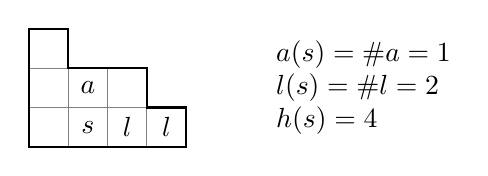
\begin{tikzpicture}[scale=.5]
\draw[thin, gray] (0,0) grid (1,3);
\draw[thin, gray] (1,0) grid (3,2);
\draw[thick] (0,0)--(0,3)--(1,3)--(1,2)--(3,2)--(3,1)--(4,1)--(4,0)--cycle;
\draw (1.5,.5) node{$s$};
\draw (1.5,1.5) node{$a$};
\draw (2.5,.5) node{$l$};
\draw (3.5,.5) node {$l$};
\draw (8.5,1.5) node[align=left] {$a(s)=\# a=1$ \\ $l(s)=\# l=2$ \\ $h(s)=4$};
\end{tikzpicture}
\end{center}
\end{example}


\begin{definition}
The \emph{hook length} of a cell $\square$, written $h(\square)$ is
$$h(\square)=a(\square)+\ell(\square)+1$$
The \emph{weighted hook length} 
$$h_k(\square)=a(\square)+k(\ell(\square)+1)$$
\end{definition}

\begin{definition}
A partition is called an $n$-core if it has no squares $\square$ with $h(\square)$ divisible by $n$.

A partition is called a $(k,n)$-core if it has no squares $\square$ with $h_k(\square)$ divisible by $n$.

We will use $\CC(k,n)$ to denote the set of all $(k,n)$ core partitions.
\end{definition}

So, an $n$-core partition is a $(1,n)$-core.  

\begin{exercise}
Show that the 2-core partitions are exactly the staircase partitions $k+(k-1)+(k-2)+(k-3)+\cdots +2+1$.
\end{exercise}



\begin{exercise}
Prove that the generating function for $(-1,3)$ cores is $1/(1-q)$ 

$$\sum_{\lambda\in\CC(-1,3)} q^{|\lambda|}=\frac{1}{1-q}$$
More explicitly, prove that for every $n$ there is exactly one partition (describe it!) of $n$ that is a (-1,3) core partition.  
\end{exercise}

\begin{OpenProblem}
Give a \emph{combinatorial} proof that
$$\sum_{\lambda\in\CC(2,5)} q^{|\lambda|}=\frac{1}{(1-q)(1-q^2)}$$
\end{OpenProblem}

I have proven something much stronger than this, but the proof uses a lot of high-power algebraic geometry.  We would like even a bijective proof.  The right hand side is the generating function for partitions where every part is size 1 or size 2, so we'd like a bijection
$$f:\N\times\N\to\CC(2,5) \quad \quad |f(x,y)|=x+2y$$
Although this is an open problem, I think it should be very doable!  I will be explaining some ideas and tools that might help with it, but it should be approachable even now, and thinking about is good practice!



\begin{question}
For a partition $\lambda$, for $k=0,1,2$ define:
$$d_{k}(\lambda)=\#\{\square\in\lambda: a(\square)-\ell(\square)=k\mod 3\}$$
and generating functions
$$\mathcal{G}_k(q,t)=\sum_{\lambda\in\mathcal{P}}q^{|\lambda|}t^{d_k(\lambda)}$$

\begin{itemize}
\item Write sage code to compute the generating functions 
\item Explain why $\mathcal{G}_1=\mathcal{G}_2$.
\item Conjecture a product formula expression for $\mathcal{G}_1$? (proving your conjecture is HARD)
\item Can you say anything about $\mathcal{G}_0$?
\end{itemize}
I haven't really thought about the last bullet point, so I'd be curious what you can find!

\end{question}
\end{document}


